\chapter{HIỆN THỰC HỆ THỐNG PHÁT HIỆN TIN NÓNG}
\ifpdf
    \graphicspath{{Chapter3/Chapter3Figs/PNG/}{Chapter3/Chapter3Figs/PDF/}{Chapter3/Chapter3Figs/}}
\else
    \graphicspath{{Chapter3/Chapter3Figs/EPS/}{Chapter3/Chapter3Figs/}}
\fi

\section{Mở đầu}
Chương này sẽ trình bày về thiết kế, chi tiết cài đặt, các thư viện và framework được sử dụng để xây dựng hệ thống phát hiện tin nóng.

\section{Mô hình hệ thống}
Dưới đây là mô hình của các thành phần chính hệ thống:
\begin{figure}[H]
	\centering
	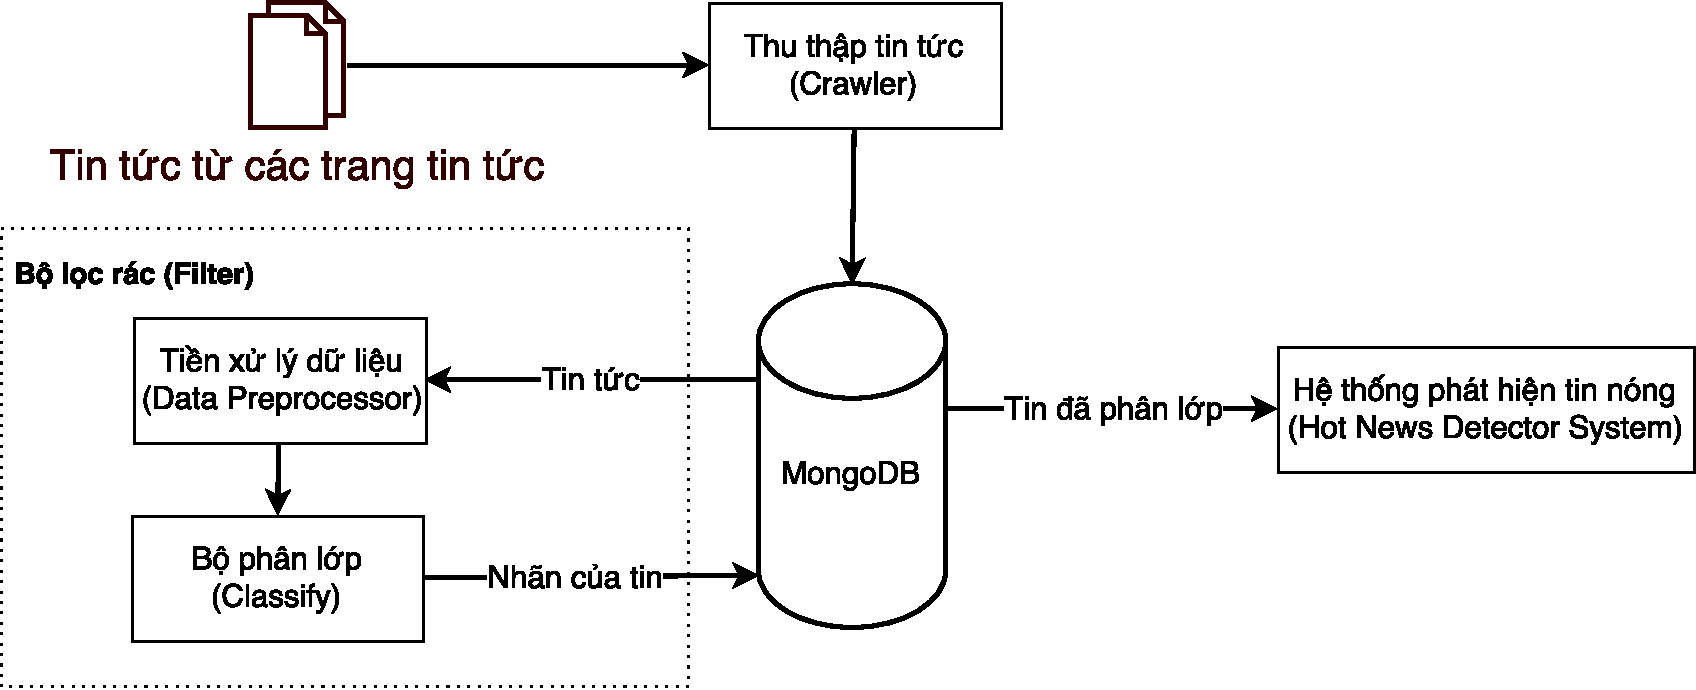
\includegraphics[width=0.9\linewidth]{Chapter3/Chapter3Figs/PDF/SystemArchitecture}
	\caption{Các thành phần chính của hệ thống}
	\label{fig:systemarchitecture}
\end{figure}

Hệ thống có 2 loại người dùng chính: quản trị viên hệ thống (admin) và biên tập viên. Quản trị viên có nhiệm vụ theo dõi hệ thống, điều khiển bật tắt, thay đổi thông số của các tác vụ trong hệ thống. Biên tập viên sử dụng hệ thống thông qua giao diện Top Stories để xem các sự kiện phát hiện được và các thông tin liên quan.
%\begin{itemize}
%	\item \textit{Data Streaming}: Module này sử dụng Twitter Streaming API để thu thập các bài đăng từ Twitter, theo một danh sách các từ khóa cho trước.
%	\item \textit{Data Preprocessor}: Module tiền xử lý (loại bỏ link, stopwords; tách từ) và biểu diễn dữ liệu thành vector trọng số tf-idf.
%	\item \textit{Clustering Algorithm}: Chạy thuật toán gom cụm trên dữ liệu đã mã hóa thành vector trọng số, đưa ra các cụm bài viết tương ứng và lưu vào cơ sở dữ liệu.
%	\item \textit{MongoDB}: Cơ sở dữ liệu chứa bài viết và các thông tin đính kèm, sử dụng MongoDB.
%	\item \textit{Top Stories}: Giao diện hiển thị các cụm tin tức đáng chú ý cho người dùng.
%\end{itemize}

\section{Phân hệ thu thập dữ liệu (Data Streaming)}
Module này sử dụng Twitter Streaming API \footnote{https://dev.twitter.com/streaming/overview} để thu thập các bài đăng từ Twitter, theo một danh sách các từ khóa cho trước. API này cho phép người dùng lấy những tweet đăng ở chế độ công khai thông qua 2 endpoint:
	\begin{itemize}
		\item GET statuses/sample: lấy mẫu ngẫu nhiên từ tất các bài đăng hiện tại.
		\item POST statuses/filter: lọc các bài theo nhiều tiêu chí cho trước như: có chứa từ khóa tìm kiếm, viết bởi ngôn ngữ nào đó, vị trí người dùng khi đăng bài, bài đăng bởi người dùng trong danh sách theo dõi. Mặc định Twitter cho phép lọc với tối đa 400 từ khóa và theo dõi tối đa 5000 người dùng.
	\end{itemize}
Cả 2 endpoint này đều có chung giới hạn: lượng tweet trả về bởi API không vượt quá 1\%\footnote{https://twittercommunity.com/t/potential-adjustments-to-streaming-api-sample-volumes/31628} tổng số tweet đang được đăng tại thời điểm đó trên Twitter. Ví dụ, với con số trung bình 6000 tweet được đăng mỗi giây vào năm 2013 \footnote{http://www.internetlivestats.com/twitter-statistics/}, mỗi giây ta có thể lấy tối đa 60 tweet. Con số này có thể dao động theo từng thời điểm.

Hệ thống sử dụng endpoint statuses/filter với 115 keywords, ngôn ngữ tiếng Việt, và thu được trung bình 2300 tweet mỗi ngày, với ngày cao nhất đạt 6329 tweet. 

\section{Phân hệ tiền xử lý dữ liệu (Data Preprocessor)}
Module tiền xử lý có nhiệm vụ chính gồm loại bỏ URL, thực hiện tách từ, loại bỏ stopwords và biểu diễn dữ liệu thành vector trọng số tf-idf. Trước khi chạy thuật toán gom cụm, dữ liệu được lấy ra từ MongoDB và tiền xử lý phần nội dung của tweet bằng các bước sau:
	\begin{enumerate}
		\item Loại bỏ URL bằng regular expression.
		\item Tách từ sử dụng thư viện TPSegmenter. Bước này dùng để biểu diễn các từ ghép trong tiếng Việt bằng cách thêm gạch nối giữa các tiếng của từ.\\
		Ví dụ: \textit{"Vụ tai nạn 13 người chết: Đã giám định mẫu máu tài xế xe tải"} qua bộ tách từ sẽ thành \textit{"Vụ tai\_nạn 13 người chết : Đã giám\_định mẫu máu tài\_xế xe\_tải"}.
		\item Loại bỏ các từ trong danh sách gồm 813 stopwords.
		\item Tính và biểu diễn dữ liệu thành vector tf-idf và metadata.
	\end{enumerate}

\section{Phân hệ thuật toán gom cụm (Clustering Algorithm)}
Chạy thuật toán gom cụm trên dữ liệu đã mã hóa thành vector trọng số, đưa ra các cụm bài viết tương ứng và lưu vào cơ sở dữ liệu. Hệ thống sử dụng thuật toán LSH cải tiến đã trình bày ở chương 2 làm thuật toán chính, với các thông số mặc định như sau:
	\begin{table}[H]
		\centering
		\setlength\extrarowheight{3pt}
		\begin{tabular}{|c|c|}
			\hline 
			Threshold & 0.5 \\ 
			\hline 
			Số hashtable & 20 \\ 
			\hline 
			Số siêu phẳng & 200 \\ 
			\hline 
			Số bài viết gần nhất để so sánh & 1000 \\ 
			\hline 
			Số bài viết tối đa cho một bucket & 200 \\ 
			\hline 
		\end{tabular} 
	\end{table}

Các thông số trên cho phép thuật toán kịp thời xử lý hết lượng dữ liệu truyền liên tục từ Twitter về, và vẫn phát hiện được các cụm tương đối tốt.

\section{Phân hệ hiển thị tin nóng (Top Stories)}
Giao diện hiển thị các cụm tin tức nóng cho người dùng. Mỗi cụm được đại diện bằng một bài viết đầu tiên, tức là bài viết sớm nhất nói về sự kiện nào đó, cùng với các thông tin như số bài viết trong cụm, tổng số favorite và retweet trong cụm, tổng số follower của người dùng có đăng bài trong cụm,... Hình \ref{fig:topstories} thể hiện giao diện đã cài đặt trên thực tế.

\section{Thiết kế hệ thống} 

	\begin{figure}[H]
		\centering
		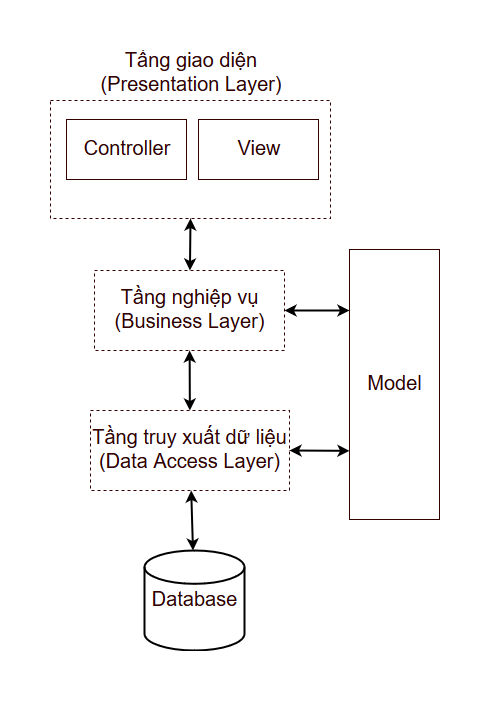
\includegraphics[width=0.5\linewidth]{Chapter3/Chapter3Figs/Layers}
		\caption{Kiến trúc hệ thống kết hợp Multilayer architecture kết hợp với mô hình MVC}
		\label{fig:layers}
	\end{figure}
Hệ thống xây dựng theo kiến trúc 3 tầng gồm: Presentation Layer, Business Logic Layer và Data Access Layer. Trong đó, Presentation Layer áp dụng mô hình Model - View - Controller (MVC). Cụ thể:
	\begin{itemize}
		\item Presentation Layer: Có trách nhiệm hiển thị thông tin, tương tác với người dùng hệ thống. Gồm 2 thành phần:
			\begin{itemize}
				\item Controller: Điều khiển các luồng của hệ thống web, nhận các tín hiệu từ người dùng và xử lý tương ứng.
				\item View: Có nhiệm vụ hiển thị các giao diện hệ thống cho người dùng.
			\end{itemize}
		\item Model: Đối tượng chứa dữ liệu để xử lý và hiển thị.
		\item Business Layer: Chứa các nghiệp vụ của hệ thống. Bao gồm các bước xử lý dữ liệu, thuật toán gom cụm, các tác vụ thống kê,...
		\item Data Access Layer: Có nhiệm vụ giao tiếp với các hệ cơ sở dữ liệu.
	\end{itemize}

\section{Cài đặt hệ thống}%các packages
Hệ thống ứng dụng được xây dựng trên nền tảng Java EE với các thành phần sau:
	\begin{itemize}
		\item Ngôn ngữ: Java, HTML, CSS, JavaScript.
		\item Hệ cơ sở dữ liệu: MongoDB và MySQL.
		\item Thư viện, framework: Apache Struts 2, Apache Lucene, TPSegmenter
		\item Server: Apache Tomcat
	\end{itemize}

	\subsection{Các package}
	Source code chương trình được tổ chức thành các package như sau:
	\begin{itemize}
		\item admicro.eds.action: Chứa các lớp action điều khiển view của Struts 2
		\item admicro.eds.bo: Chứa các business object của hệ thống
		\item admicro.eds.clustering: Chứa các lớp của thuật toán gom cụm
		\item admicro.eds.config: Các file config cho hệ thống
		\item admicro.eds.constant: Các hằng số dùng chung trong chương trình
		\item admicro.eds.crawler: Duyệt các trang tin được chia sẻ trong tweet và lấy thêm thông tin bổ sung
		\item admicro.eds.dao: Data Access Object, thực hiện các tác vụ đọc, ghi database
		\item admicro.eds.dbconnection: Cung cấp kết nối đến database
		\item admicro.eds.dto: Data Transfer Object, các đối tượng để vận chuyển dữ liệu từ database
		\item admicro.eds.interceptor: Chứa các lớp interceptor của Struts 2
		\item admicro.eds.lucene: Gồm các tác vụ sử dụng thư viện Apache Lucene như index dữ liệu, tính toán tf-idf,...
		\item admicro.eds.statistics: Chạy thống kê dữ liệu offline
		\item admicro.eds.thread: Các lớp bao đóng để tạo thread chạy song song các tác vụ
		\item admicro.eds.utility: Các công cụ hỗ trợ trong hệ thống
	\end{itemize}
	
	\subsection{Cơ sở dữ liệu MongoDB}
	Hệ thống sử dụng MongoDB để lưu trữ dữ liệu tin tức và quản lý kết quả gom cụm. Đây là một hệ cơ sở dữ liệu NoSQL, cung cấp khả năng mở rộng, sao lưu, phân mảnh dữ liệu tốt, và có thể thay đổi cấu trúc dữ liệu một cách linh hoạt.
	
	Dưới đây là bảng so sánh một số thuật ngữ cơ bản giữa các cơ sở dữ liệu SQL truyền thống và MongoDB:
	\begin{table}[H]
		\centering
		\setlength\extrarowheight{3pt}
		\begin{tabular}{|l|l|}
			\hline
			\textbf{Thuật ngữ SQL}	& \textbf{Thuật ngữ MongoDB}  \\\hline
			database	& database \\\hline
			table		& collection \\\hline
			row			& document hoặc BSON document \\\hline
			column		& field \\\hline
			index		& index \\\hline
			table joins	& \$lookup, embedded documents \\\hline
		\end{tabular}
		\caption{So sánh các thuật ngữ giữa SQL và MongoDB}
		\label{tab:table_3_1}
	\end{table}
	
		\subsubsection{Collection Streaming}
		Collection này chứa thông tin về các bài viết thu thập được từ Twitter, cũng là nơi lưu trữ tất cả thông tin về tweet trong hệ thống. Khi dữ liệu được stream từ Twitter về, mỗi tweet chỉ có 8 trường, các trường khác sẽ được thêm vào trong quá trình hệ thống xử lý.
		\begin{table}[H]
			%				\centering
			\setlength\extrarowheight{3pt}
			\begin{tabular}{|l|l|p{7.25cm}|}
				\hline
				\textbf{Thuộc tính}     & \textbf{Loại} & \textbf{Ý nghĩa} \\\hline
				\_id           & ObjectID       & ID trong MongoDB của document \\\hline
				TweetID        & Long           & ID của tweet do Twitter tạo ra\\\hline
				UserID         & Long           & ID của người dùng Twitter\\\hline
				UserScreenName & String         & Tên tài khoản của người dùng Twitter \\\hline
				TweetContent   & String         & Nội dung của tweet, bao gồm nội dung chữ và đường link được chia sẻ\\\hline
				TweetPostDate  & Date           & Thời gian đăng của tweet\\\hline
				CollectDate    & Date           & Thời gian tweet được thu thập vào hệ thống\\\hline
				FavoriteCount  & Integer        & Số lượng favorite của tweet\\\hline
				RetweetCount   & Integer        & Số lượng retweet của tweet\\\hline
				TrackingNumber & Integer        & \\\hline
				LinkPostDate   & String         & Ngày đăng của bài viết được share trong tweet (nếu có)\\\hline
				clusterID      & Integer        &  ID cụm mà tweet được phân vào, là TweetID của tweet đại diện cụm\\\hline
				category       & String         & Chủ đề của tweet\\\hline
				breakingLabel  & String         & Nhãn phân lớp của Tweet sau khi chạy bộ phân lớp\\\hline
				probabilityForNo & Double       & Xác suất tweet thuộc lớp "Không" (nóng)\\\hline
				probabilityForIrrelevant & Double         &  Xác suất tweet thuộc lớp "Không liên quan"\\\hline
				probabilityForYes & Double         &  Xác suất tweet thuộc lớp "Có" (nóng)\\\hline
				feedback      & String        & Phản hồi về nhãn phân lớp của biên tập viên\\\hline
				
			\end{tabular}%
			
			\caption{Các trường của collection Streaming}
			\label{tab:table_3_2}%
		\end{table}%
		
		\subsubsection{Collection Cluster}
		Collection cluster chứa thông tin các cụm bài viết. Mỗi Mongo document là một cụm và bao gồm các thông tin tổng quan của cụm.
		\begin{table}[H]
			%				\centering
			\setlength\extrarowheight{3pt}
			\begin{tabular}{|l|l|p{9cm}|}
				\hline
				\textbf{Thuộc tính}     & \textbf{Loại} & \textbf{Ý nghĩa} \\\hline
				\_id           & ObjectID       &  ID trong MongoDB của cụm\\\hline
				ClusterID      & Long           &  ID cụm, là TweetID của tweet đại diện cụm\\\hline
				Size	       & Long           &  Số bài viết trong cụm\\\hline
				TotalFavorite	& String         & Tổng số favorite của các tweet trong cụm\\\hline
				TotalRetweet	& String         & Tổng số retweet của các tweet trong cụm\\\hline
				TotalFollower	& String         & Tổng số người theo dõi của những người đăng bài trong cụm\\\hline
				RankingScore	& String         & Điểm xếp hạng của cụm\\\hline
				
			\end{tabular}%
			\caption{Các trường của collection Cluster}
			\label{tab:table_3_3}%
		\end{table}%

	\subsection{Cơ sở dữ liệu MySQL}
	MySQL được dùng để lưu trữ các dữ liệu khác của hệ thống như dữ liệu người dùng, các từ khóa dùng cho việc streaming dữ liệu Twitter,...
		\subsubsection{Bảng User}
		Bảng này dùng để quản lý danh sách người dùng hệ thống.
			\begin{table}[H]
				\centering
				\setlength\extrarowheight{3pt}
				\begin{tabular}{|l|l|l|}
					\hline
					\textbf{Thuộc tính} & \textbf{Loại} & \textbf{Ý nghĩa} \\ \hline
					ID & int(11) & ID của người dùng\\\hline
					Username & varchar(100) &  Tên tài khoản\\\hline
					Password & Long &  Mật khẩu\\\hline
					Email & varchar(100) &  Địa chỉ email người dùng\\\hline
					Fullname & varchar(100) &  Họ tên đầy đủ của người dùng\\\hline
					Phone & varchar(20) &  Số điện thoại\\\hline
					UserTypeId & int(11) &  ID phân loại người dùng\\\hline
				\end{tabular}
				\caption{Bảng User}
				\label{tab:usertable}
			\end{table}
	
		\subsubsection{Bảng UserType}
		Bảng chứa thông tin loại người dùng.
			\begin{table}[H]
				\centering
				\setlength\extrarowheight{3pt}
				\begin{tabular}{|l|l|l|}
					\hline
					\textbf{Thuộc tính} & \textbf{Loại} & \textbf{Ý nghĩa} \\\hline
					ID      	& int(11)           &  Khóa chính của bảng\\\hline
					UserType	& varchar(100)      &  Loại tài khoản (admin hay biên tập viên)\\\hline

				\end{tabular}
				\caption{Bảng UserType}
				\label{tab:usertypetable}
			\end{table}
		
		\subsubsection{Bảng Topic}
		Bảng chứa danh sách từ khóa cho việc stream dữ liệu từ Twitter về
			\begin{table}[H]
				\centering
				\setlength\extrarowheight{3pt}
				\begin{tabular}{|l|l|l|}
					\hline
					\textbf{Thuộc tính}     & \textbf{Loại} & \textbf{Ý nghĩa} \\\hline
					ID      	& int(11)       &  Khóa chính của bảng\\\hline
					Topic	& varchar(100)      &  Tên chủ đề\\\hline
					Keyword	& varchar(1000)    	&  Danh sách từ khóa\\\hline
				\end{tabular}
				\caption{Bảng Topic}
				\label{tab:topic}
			\end{table}
\section{Kết quả}
Hệ thống đã hoàn thiện các chức năng: Thu thập dữ liệu từ Twitter, điều khiển chạy luồng của thuật toán phát hiện tin nóng, và hiển thị kết quả cho biên tập viên. Dưới đây là một số hình ảnh của hệ thống:

\begin{figure}[H]
	\centering
	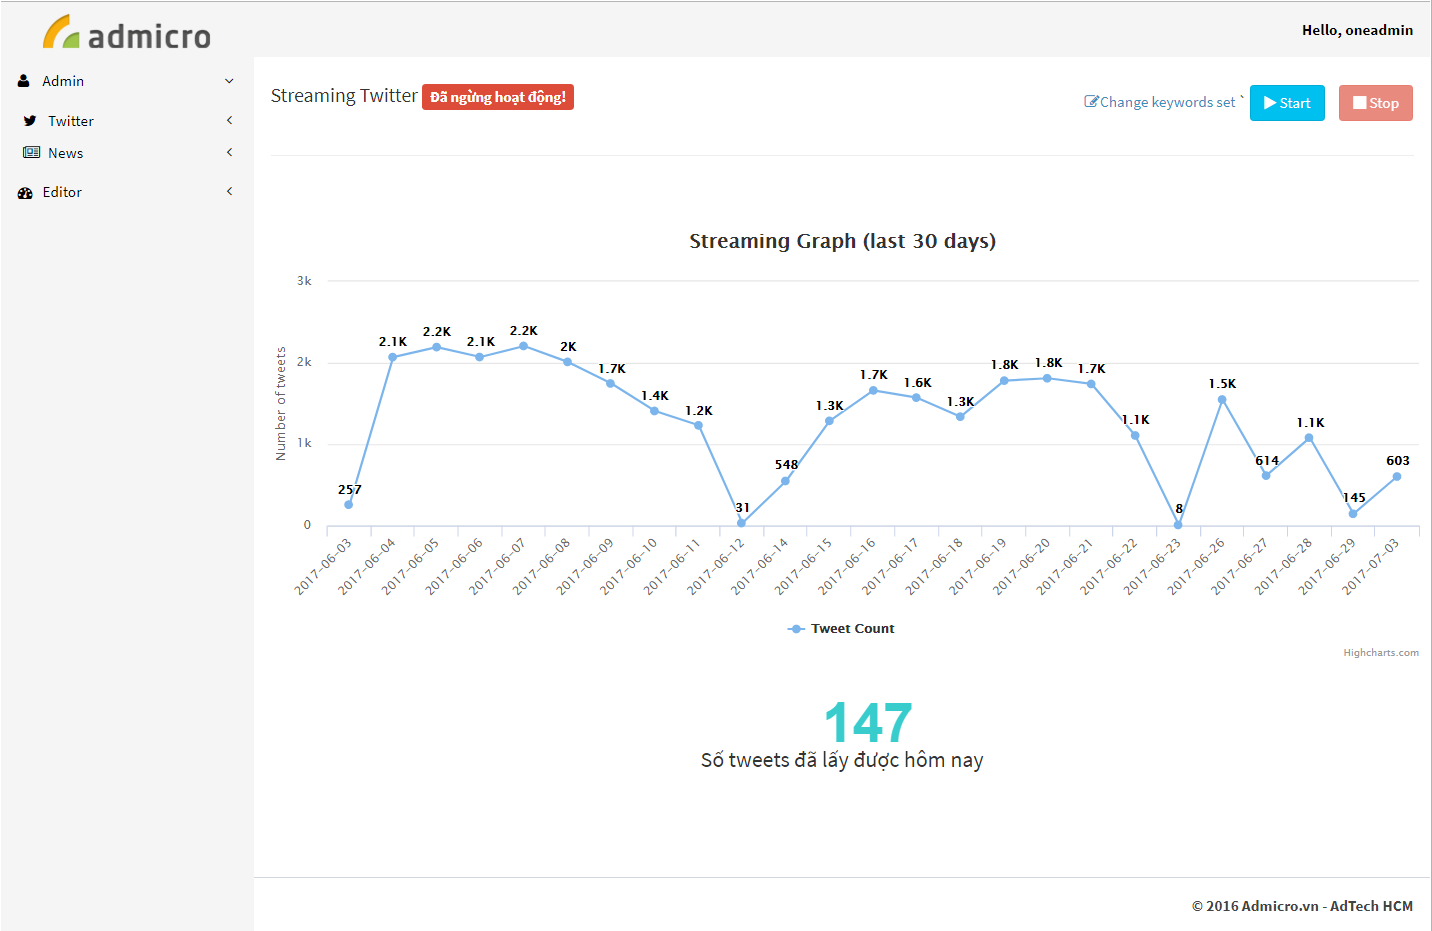
\includegraphics[width=1\linewidth]{Chapter3/Chapter3Figs/StreamingNonwide}
	\caption{Giao diện điều khiển thu thập dữ liệu Twitter}
	\label{fig:streaming}
\end{figure}

\begin{figure}[H]
	\centering
	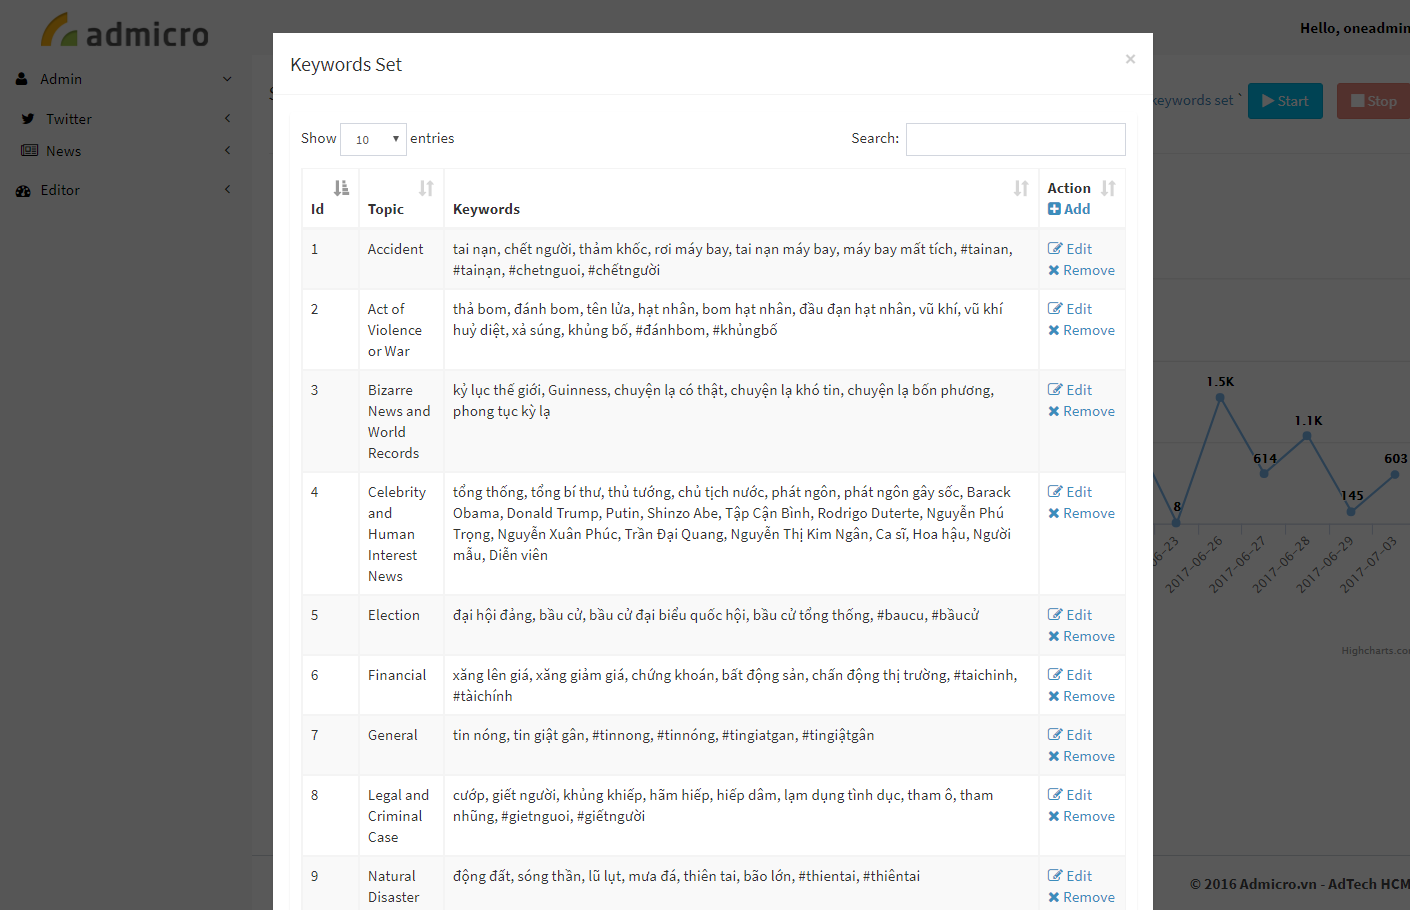
\includegraphics[width=0.96\linewidth]{Chapter3/Chapter3Figs/StreamingKeywords}
	\caption{Giao diện thêm xóa từ khóa để thu thập dữ liệu Twitter}
	\label{fig:streamingkeywords}
\end{figure}

\begin{figure}[H]
		\centering
	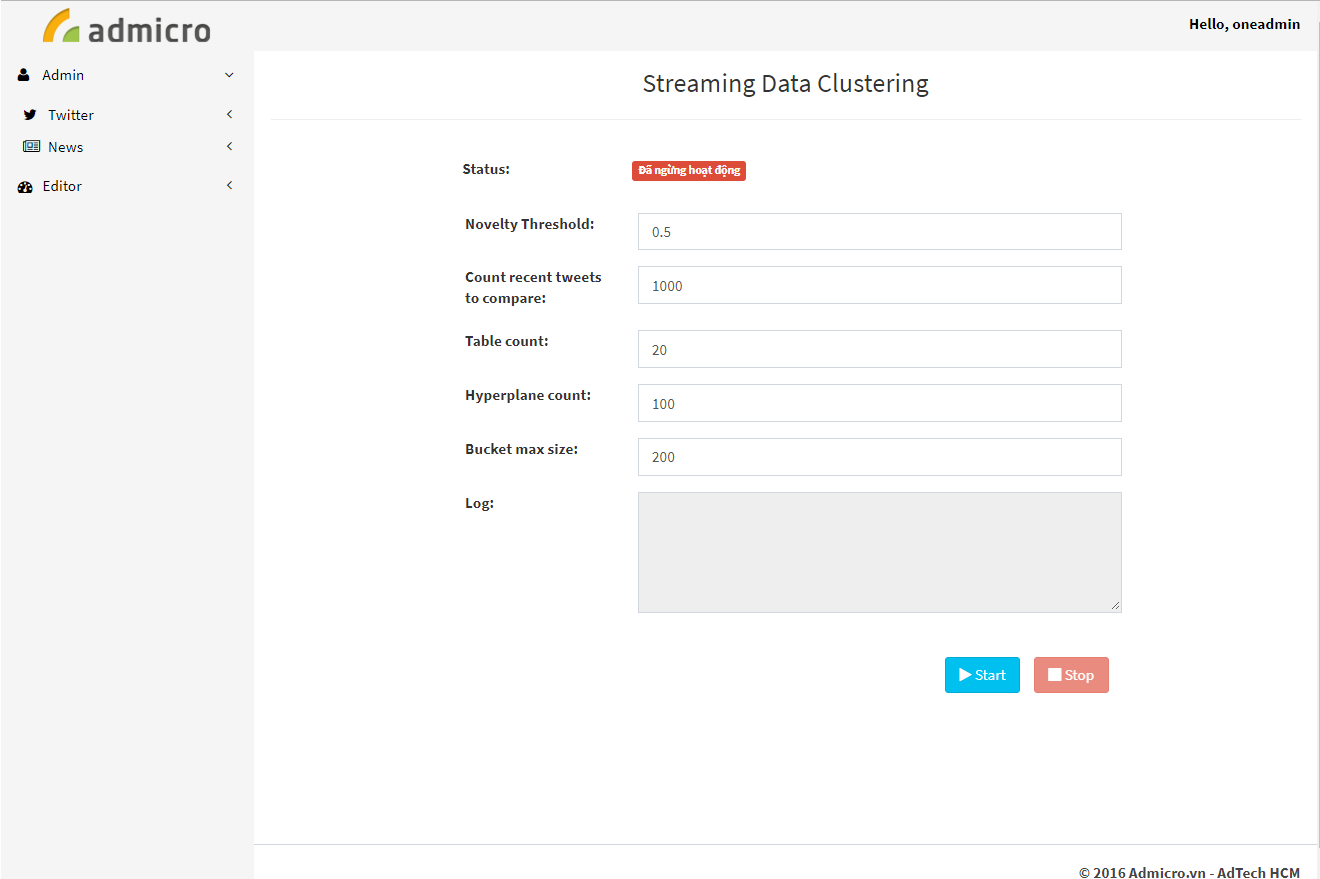
\includegraphics[width=0.96\linewidth]{Chapter3/Chapter3Figs/StartClustering}
	\caption{Giao diện điều khiển thuật toán phát hiện tin nóng}
	\label{fig:startclustering}
\end{figure}

\begin{figure}[H]
		\centering
	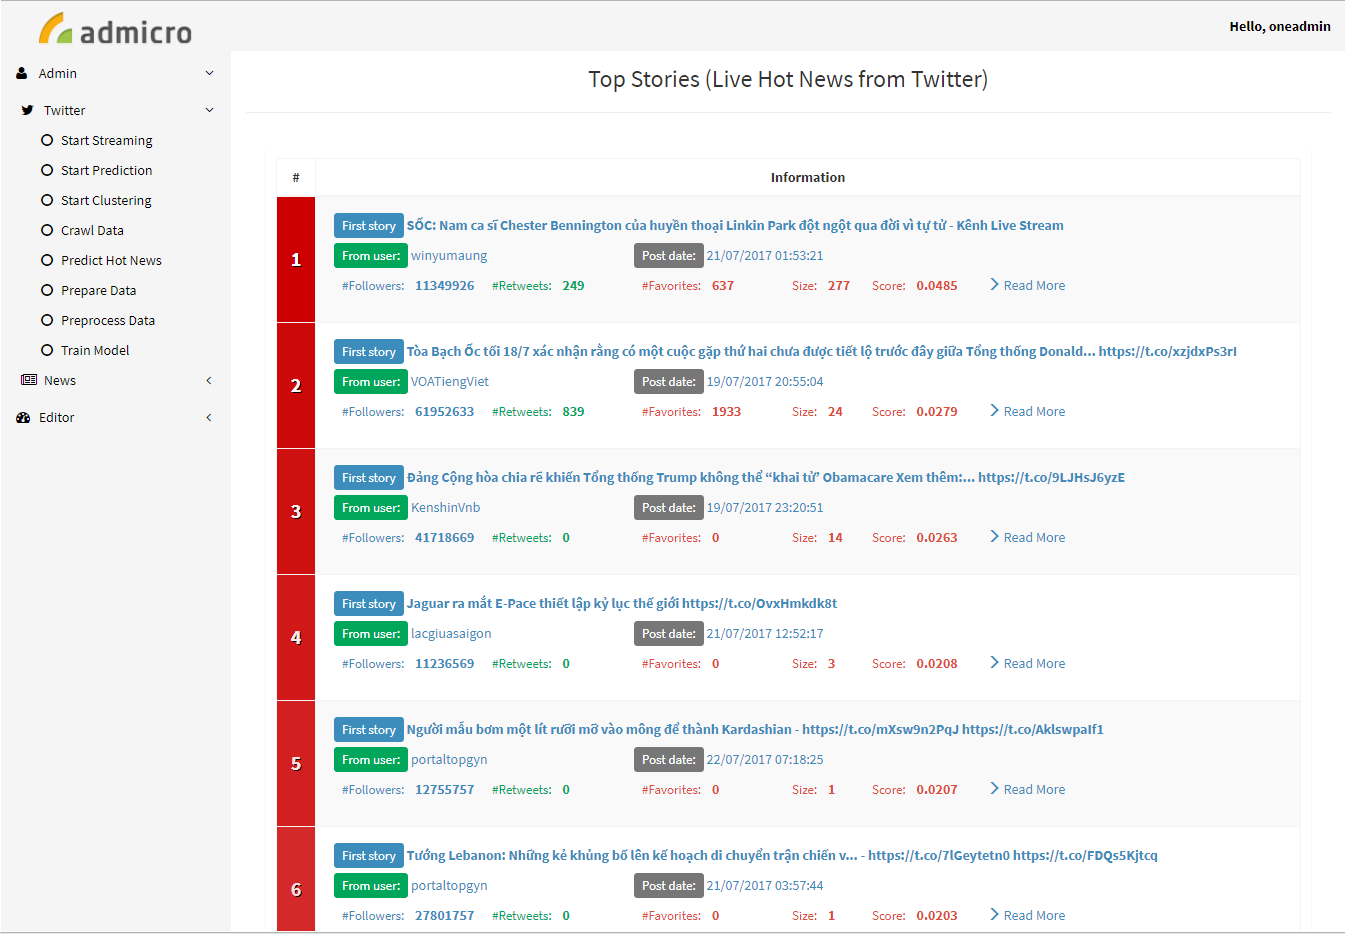
\includegraphics[width=0.96\linewidth]{Chapter3/Chapter3Figs/TopStories2}
	\caption{Giao diện hiển thị các cụm bài viết cho biên tập viên}
	\label{fig:topstories}
\end{figure}

\begin{figure}[H]
	\centering
	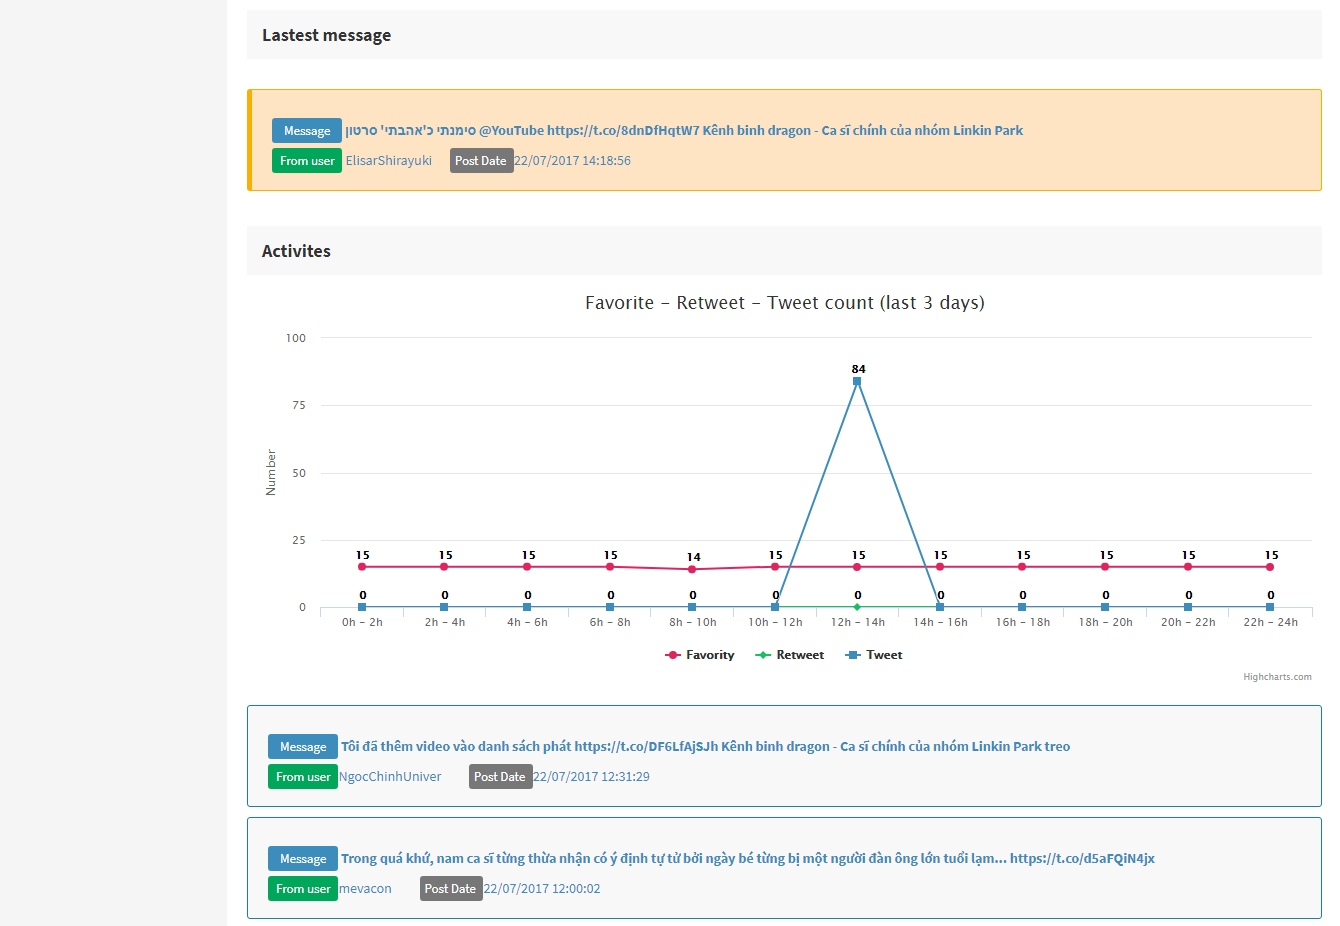
\includegraphics[width=0.96\linewidth]{Chapter3/Chapter3Figs/StoryDetails2}
	\caption{Chi tiết một cụm bài viết}
	\label{fig:storydetail}
\end{figure}

\section{Kết chương}
Chương này đã trình bày về các thành phần chính hệ thống, kiến trúc phân tầng, các hệ cơ sở dữ liệu được sử dụng và cách tổ chức, cùng một số kết quả cài đặt hệ thống.